
\chapter{Fourier transform on a finite group}
\label{chap-transforme-fourier-finite-group}



In this first chapter, we will approach the study of the Fourier transform from an original angle, that of group theory. Fourier theory, whether viewed from an algebraic point of view or not, consists above all in the analysis of functions. Here we must take the word analysis literally, in its etymological sense. It's about breaking down complex data into a simpler form. It will therefore be a question of constructing a systematic means to obtain this decomposition, and this is precisely where the Fourier tools come into play. To achieve this decomposition efficiently, we must still use a certain amount of a priori information about the functions we are studying. This first chapter will relate to the study of functions on a finite group; the \guill{elementary bricks} decomposition carried out by the Fourier analysis will result from the symmetries inherent in the group structure. \index{Symmetry}

The most elementary framework to carry out this project is that of finite commutative groups, since one does not have to worry about either the regularity of the functions encountered, or the convergence of the manipulated series (since they are finite!). Of course, one will be tempted to cry scandal as the work then accomplished seems simplistic compared to the \guill{analytic} theory of Fourier series. However, this study makes it possible to bring new points of view and to pose new questions which will be addressed in the next chapters.
\begin{rs}
\item How can the study of the Fourier transform on a finite group help us to understand the construction of the continuous Fourier transform?
\item How does the Fourier transform on finite groups join the discrete Fourier transform?
\item What uses can we make of the Fourier transform on a finite group? How to build efficient algorithms, and how to implement them?
\item Finally, what happens to this theory when we try to apply it to non-commutative groups? This question will motivate the introduction of new tools, described in detail in the last two chapters.
\end{rs} It is to this set of questions that we will try to answer. The methods implemented are multiple, they often borrow from several mathematical disciplines.

There are many references to the subject of duality on finite groups. There is of course the book of \nompropre{J.P.Serre} \cite{serre}, but also for example that of \nompropre{Warusfel} \cite{warusfel}, for a more detailed presentation. For an introduction to the Fourier transform on a commutative group, we can look at the work of \nompropre{Dym} and \nompropre{Mac Kean} \cite{dym}.

% ------------------------------------------------- -----
% ------------------------------------------------- -----
% ------------------------------------------------- -----
% section - Dual of a finite group
% ------------------------------------------------- -----
% ------------------------------------------------- -----
% ------------------------------------------------- -----
\section{Dual of a finite group}
% \addcontentsline{toc}{section}{Dual of a finite group}
\label{sect1-dual-group}

The aim of this book is to study, from an algebraic point of view, the functions with complex values whose starting space is a finite group denoted by $G$. It is a question of making maximum use of the properties of the group to obtain interesting functional decompositions. The basic idea of this chapter, the one which will guide our reflections until the end of this book, consists in studying how we can represent a function on a group $G$. The generally most common way to think about a function $ f: G \rightarrow \CC$ is to consider the set of its values $ f(g)$ for $ g \in G$. The major disadvantage of this representation is that it does not exploit the structure of our group $G$ at all. In a way, it is a universal representation, which does not depend at all on the group that one has chosen. To study a function efficiently, it seems logical to build a new representation that exploits the symmetries that can be found in a group $G$. The simplest example of these symmetries is the cyclic character of the group $\ZZ/n\ZZ$, but we can of course consider more complex constructions.

% ------------------------------------------------- -----
% ------------------------------------------------- -----
% sub-section - Definitions
% ------------------------------------------------- -----
% ------------------------------------------------- -----
\subsection{Definitions}

\index{Subgroup} To understand how a function can be more or less simple to represent, we will first approach the simplest functions, those which do not oppose any resistance to the structure of the starting group $G$. We are therefore going to focus on the functions that carry the structure of the group. These functions are the morphisms of the group $G$ into a group of the arrival set, that is, a subgroup of $\CC^*$. We will therefore introduce the appropriate definitions.

\begin{defn}[Characters and dual of a group]
\label{notation-0} \label{notation-1} \index{Dual!of a finite abelian group} \index{Character!of an abelian group} \index{Duality!on a group} Let $G$ a finite group. By definition, a \textit{character}$\chi$ is a morphism from the group $G$ into the multiplicative group $\CC^*$. We denote by $\wh{G}$ the set of characters, which we call the \textit{dual} of $G$.
\end{defn}
$\wh{G}$ is a group for multiplication of applications. It is recalled that this multiplication is defined as follows.
\begin{equation*}
\forall(\chi_1, \, \chi_2) \in \wh{G}^2, \quad \chi_1 \chi_2: x \mapsto \chi_1 (x) \chi_2 (x).
\end{equation*}
We will see, in particular in Paragraph~\ref{sect2-bidual}, that the duality over a finite group has many points in common with the duality between vector spaces. In the next chapter, more precisely in Paragraph~\ref{abelian-finite-grpe-fish-formula}, we will even see that in certain cases, this rapprochement can become an identity between the two structures (of group and of vector space). The duality on a finite group then makes it possible to demonstrate interesting linear properties. In the meantime, let's start by studying the image of a character $\chi \in \wh{G}$.

\begin{prop}
\label{prop-pte-elem-car}
\index{Morphism!character} \label{notation-2} \label{notation-3} \label{notation-4} \label{notation-5} Let $G$ be a finite group of cardinal $|G| = n $. The elements of $\wh{G}$ are in fact the morphisms of $G$ in the group of the \ordin{n}{ith} roots of the unit,
\begin{equation*}
\UU_n = \left\{\exp \left(\frac{2 \imath k \pi}{n} \right) \; \bigg \backslash \; 0 \leq k <n \right\}.
\end{equation*}
In particular,
\begin{equation*}
\forall g \in G, \quad |\chi(g) | = 1, \quad \chi(g^{-1}) = \chi(g)^{-1} = \ol{\chi(g)},
\end{equation*}
where we denote by $|z|$ the modulus of a complex number $ z $, and $\ol{z}$ its conjugate.
\end{prop}

\begin{proof}
\index{Root!of unit} Denote by $ 1$ the neutral element of $G$. Note that for any element $ g \in G$, we have $ g^n = 1$. This therefore implies, for all $\chi \in \wh{G}$, that $\chi(g)^n = \chi(g^n) = 1$, which means that $\chi$ is at values in the set of \ordin{n}{th} roots of the unit.
\end{proof}


\begin{rem}
It follows that in particular, $\wh{G}$ is a finite group (because there is only a finite number of maps of $G$ in $\UU_n$, which are finite sets) , commutative. Moreover, every element $\chi \in \wh{G}$ is constant over the conjugation classes of $G$, since
\begin{equation}
\label{eq-character-constant-class-conjug}
\forall (g, \, h) \in G^2, \quad \chi(h^{-1} gh) = \chi(h)^{-1} \chi(g) \chi(h) = \chi(e) \chi(g) = \chi(g).
\end{equation}
\end{rem}


\begin{defn}[Function space on $\mbold{G}$]
\label{defn-space-function-g-in-c}
\index{Space!of functions of $G$ in $\CC$} \label{notation-6} \label{notation-7} We denote by $\CC[G]$ the set of functions of $G$ in $\CC$. The notation $\CC[G]$ will be explained in Paragraph~\ref{sect2-algebre-grpe-abelien}. It is a vector space on $\CC$. We define a Hermitian dot product, by \label{notation-8} \label{notation-9} \label{notation-10}
\begin{equation}
\label{eq-defn-prod-herm-c-g-abelien}
\forall (f, \, g) \in \CC[G]^2, \quad \dotp{f}{g} \eqdef \frac{1}{|G|} \sum_{x \in G}{f (x) \ol{g (x)}}.
\end{equation}
We also define a norm $\norm{\cdot}_2 $ on $\CC[G]$ by $\norm{f}_2^2 \eqdef \dotp{f}{f}$.
\end{defn}


\begin{rem}
\label{notation-11} \index{Translation} The Hermitian product that we have just defined on $\CC[G]$ presents strong similarities with the one that can be defined between two functions of $L^2(\RR)$ as follows:
\begin{equation*}
\forall (f, \, g) \in L^2(\RR)^2, \quad \dotp{f}{g} = \int_{\RR}{f (x) \ol{g (x)} \d x}.
\end{equation*}
The main difference is the change of the sum to integral. One of the common properties of these two dot products is translational invariance. Indeed, if we denote by $ T_y (f)$ the function $ x \in G \mapsto f (xy) \in G$ (or its continuous analogue $ T_y (f) = f(\cdot + y)$), we have
\begin{equation*}
\dotp{T_h (f)}{T_h(g)} = \dotp{f}{g}.
\end{equation*}
This property will be constantly used thereafter, among other things to demonstrate the orthogonal relations between characters.
\end{rem}
In order to study the functions of $\CC[G]$, we will introduce a canonical basis. The decomposition in this base corresponds to the standard way of representing a function of a set in $\CC$.

\begin{prop}
\label{prop-base-c-g}
\index{Base!of $\CC[G]$} A basis of $\CC[G]$ is given by the following $(\delta_g)_{g \in G}$ functions:
\begin{equation}
\label{eq-defn-delta-function-g}
\delta_g(h) \eqdef \left\{\begin{array}{lll} 1 & \text{if} & h = g \\0 & \text{if} & h \neq g \end{array} \right. .
\end{equation}
In particular, $\CC[G]$ is a vector space of dimension $n = |G|$ on $\CC$.
\end{prop}
\begin{proof}
We immediately check that the family is orthonormal for the Hermitian product \eqref{eq-defn-prod-herm-c-g-abelien}. As these functions are not zero, this implies that they form a free family of $\CC[G]$. The fact that this family is also a generator comes from the canonical decomposition
\begin{equation}
\label{eq-decomposition-c-g-dirac-abelien}
\forall f \in \CC[G], \quad f = \sum_{g \in G}{f(g) \delta_g},
\end{equation}
which ends the demonstration.
\end{proof}
This proposition allows to immerse $G$ in $\CC[G]$ in a canonical way by $ g \mapsto \delta_G$. Moreover, we have seen that any function $ f \in \CC[G]$ decomposes in the base $\{\delta_g\}_{g \in G}$, this is what the equation expresses \eqref{eq-decomposition-c-g-dirac-abelien}. This decomposition is apparently very simple. We will however see in Paragraph~\ref{sect2-convolution-transforme-fourier}, with the notion of \textit{convolution}, that it does not facilitate calculations at all. This is why we are going to look for a database which has the following two properties. 
\begin{rs}
\item It must be easy to use (the decomposition in this base must be easy to calculate).
\item It must have interesting properties for the algebraic operations that we want to use (linear combination, product, and product of convolution of functions).
\end{rs} 
The character family, formed from the elements of $\wh{G}$, might be a good candidate; it remains to be shown that she possesses the required qualities.

% ------------------------------------------------- -----
% ------------------------------------------------- -----
% sub-section - Dual of a cyclic group
% ------------------------------------------------- -----
% ------------------------------------------------- -----
\subsection{Dual of a cyclic group}
\label{sect1-dual-cyclic-group}


Before launching into the general study of duality on any group, let's take the time to see how all this behaves in the simplest case, that of a cyclic group (whose archetype is $\ZZ/n\ZZ$, for a given integer $n$). In fact, this example is of prime importance, on the one hand because in practice, it is the structure that we meet most often (we will see in chapter \oldref{chap-tfd} that unidimensional calculations in signal processing use the structure of $\ZZ/n\ZZ$), and secondly because we will use these results to demonstrate the general case.

\begin{prop}[The cyclic case]
\label{prop-cyclic-case}
\index{Group!cyclic} Let $ G = \{1, \, g_0, \, g_0^2, \ldots, \, g_0^{n-1}\}$ be a cyclic group of cardinal $n$ and generator $ g_0 $. \label{notation-12} Let $\omega $ be a primitive root \ordin{n}{th} of the unit, for example $\omega = e^{\frac{2 \imath \pi}{n}}$. The elements of $\wh{G}$ are of the form, for $ j \in \{0, \ldots, \, n-1\}$,
\begin{equation*}
\chi_j: \func{G}{\CC^*}{g = g_0^k}{(\omega^j)^k = e^{\frac{2 \imath \pi j k}{n}}}.
\end{equation*}
\label{notation-13} In particular, we have $ G \simeq \wh{G}$.
\end{prop}
\begin{proof}
To determine a character $\chi \in \wh{G}$, we need to calculate the value of $\chi(g_0^k)$, for $ k \in \{0, \ldots, \, n-1\}$, which gives
\begin{equation*}
\chi(g_0^k) =(\omega^j)^k = \omega^{j k}.
\end{equation*}
In this equality, we have noted $\omega^j \eqdef \chi(g_0)$, with $0 \leq j \leq n-1$, since, as we have seen in the proposition \ref{prop-pte-elem-car}, this quantity is a \ordin{n}{th} root of the unit. So our character $\chi \in \wh{G}$ is indeed one of $\{\chi_0, \ldots, \, \chi_{n-1}\}$. Conversely, we see that, for $ j \in \{0, \ldots, \, n-1\}$, the maps $\chi_j $ are indeed morphisms from $G$ into $\CC^*$, so are indeed elements of $\wh{G}$. \\Finally, if we identify the elements of $\ZZ/n\ZZ$ and their representatives in $\{0, \ldots, \, n-1\}$, we define an application $\psi: j \mapsto \chi_j $ from $\ZZ/n\ZZ$ in $\wh{G}$. We saw that this application was surjective. On the other hand, this application is injective (it suffices to evaluate $\chi_j = \psi (j)$ in $ g_0 $) and it is a morphism (elementary verification). It is therefore an isomorphism and therefore $\wh{G}$ is isomorphic to $\ZZ/n\ZZ$, itself isomorphic to $G$.
\end{proof}
The figure \figref{fig-cyclic-characters} shows the first four characters of the group $\ZZ/12 \ZZ$. On the x-axis, we have denoted $\{0, \ldots, \, 11\}$ the representatives of the group $\ZZ/12 \ZZ$, and the character values are denoted $ *$. The top line shows the real parts of the characters, and the bottom line the imaginary parts. We can see that the points are regularly spaced along the curves of equations $ y = \cos \left(\frac{2 \pi}{N} x \right)$ and $ y = \sin \left(\frac{2 \pi}{N} x \right)$.

\begin{figure}[ht]
    \begin{center}
    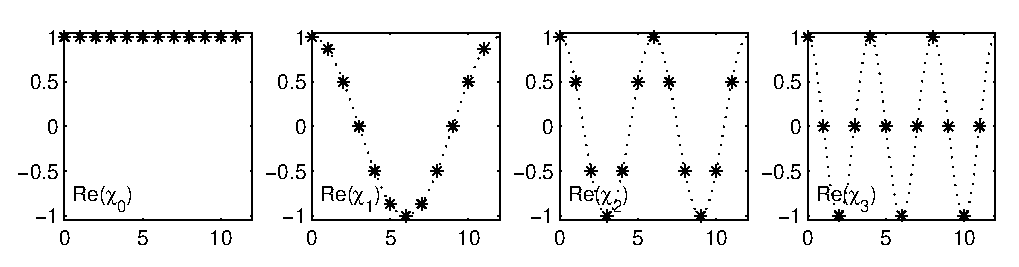
\includegraphics[scale=.7]{images/caracteres-cycliques-1.eps}
    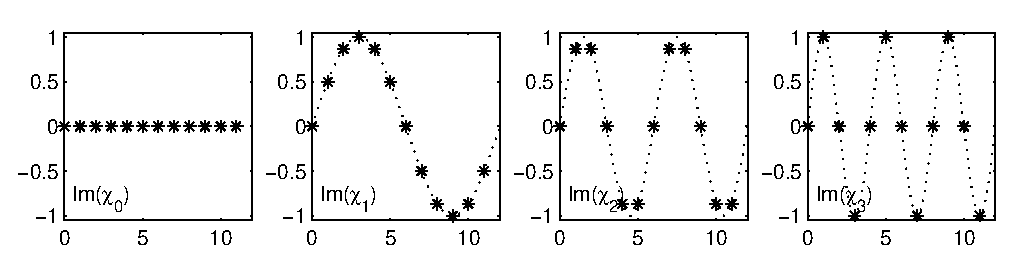
\includegraphics[scale=.7]{images/caracteres-cycliques-2.eps}
    \end{center}
    \caption{The first four characters of the group $\ZZ/12\ZZ$}
\label{fig-cyclic-characters}
\end{figure}


\begin{rem}
We can already notice that this isomorphism is not canonical, since it depends on the choice of the primitive root of the unit $\omega $ chosen. This phenomenon is recurrent in the study of duality (we find it in the linear duality between vector spaces), the dual not being canonically isomorphic to the starting group. All this will be specified later, in particular in Paragraph~\ref{sect2-bidual}.
\end{rem}


\begin{rem}
\label{rmk-zpz-isomorphism}
\index{Isomorphism!between $G$ and $\wh{G}$} Any cyclic group is isomorphic to $\ZZ/n\ZZ$ for $n = |G|$. In a way, the study of the duality on the group $\ZZ/n\ZZ$ sums up the one that we can do on any other cyclic group. In the remainder of the presentation, we will consider groups built from the elementary bricks that are groups of the type $\ZZ/n\ZZ$. This is why we must keep in mind the structure of duality on these particularly simple groups. By applying the proposition \ref{prop-cyclic-case}, we obtain the isomorphism that must be retained:
\begin{equation*}
\forall n \in \NN^*, \quad \wh{\ZZ/n\ZZ} \simeq \ZZ/n\ZZ.
\end{equation*}
We will see that in fact this property extends to any finite commutative groups.
\end{rem}


Before closing this paragraph, notice that we have $|\wh{G}| = |G| = \dim_{\CC}(\CC[G])$. We even have a stronger property.

\begin{prop}
\label{prop-base-ortho-cyclic-case}
\index{Base!orthogonal} Let $G$ be a cyclic group. $\wh{G}$ forms an orthonormal basis of $\CC[G]$, which means that
\begin{equation*}
\forall (p, \, q) \in \{0, \ldots, \, n-1\}^2, \quad \dotp{\chi_p}{\chi_q} = \delta_p^q,
\end{equation*}
where we define the symbol of \textit{Kroneker}$\delta_p^q $ as follows:
\begin{equation*}
\delta_p^q = \left\{\begin{array}{ccc} 0 & \text{if} & p \neq q \\1 & \text{if} & p = q \end{array} \right. .
\end{equation*}
\index{Kroneker's!symbol} \label{notation-14}
\end{prop}

\begin{proof}
We can assume that $ G = \ZZ/n\ZZ$. \\We write $\wh{G} = \{\chi_i\}_{i = 0}^{n-1}$, with $\chi_i (k) = \omega^{ik}$, where $\omega $ is a primitive \ordin{n}{ième} root (according to the proposition \ref{prop-cyclic-case}). We then have
\begin{equation}
\label{eq-orthogonalite-cyclic-case}
\forall (p, \, q) \in \{0, \ldots, \, n-1\}^2, \quad \dotp{\chi_p}{\chi_q} = \frac{1}{n} \sum_{i = 0}^{n-1}{(\omega^{pq})^{i}} = \delta_p^q
\end{equation}
(we obtain the last equality by summing the geometric series of reason $\omega^{p-q}$). \\The family $\wh{G} = \{\chi_i\}_{i = 0}^{n-1}$ is therefore orthonormal, and therefore in particular free. To conclude that it does indeed form a base, it suffices to notice that its cardinality is equal to the dimension of $\CC[G]$, since we have seen that $|G| = |\wh{G}|$.
\end{proof}


\begin{rem}
The proof of the orthogonality of the characters in the general case of an abelian group is hardly more complicated, and will be exposed to the proposition \ref{prop-orthogonalite-car-grpe-abelien}. However, the proof that we have just made is essential since it is at the base of the results of the one-dimensional Fourier transform, which will be presented in the Section~\ref{sect1-language-processing-signal}.
\end{rem}

% ------------------------------------------------- -----
% ------------------------------------------------- -----
% ------------------------------------------------- -----
% section - Dual of an abelian group
% ------------------------------------------------- -----
% ------------------------------------------------- -----
% ------------------------------------------------- -----
\section{Dual of an abelian group}
% \addcontentsline{toc}{section}{Dual of an abelian group}
\label{sect1-dual-abelien-group}

Our goal is to extend the result we have just demonstrated ($\wh{G}$ is an orthonormal basis of $\CC[G]$) to any finite abelian group. To achieve this, we will use a purely algebraic approach, which uses a character extension theorem. Then, we will establish a stronger result, namely that we have in fact an isomorphism between $\wh{G}$ and $G$, property that once again we have proved in the case of cyclic groups .
% ------------------------------------------------- -----
% ------------------------------------------------- -----
% sub-section - Algebraic approach
% ------------------------------------------------- -----
% ------------------------------------------------- -----
\subsection{Algebraic approach}
\label{sec2-approach-algebraic-dual-abelien}

The following lemma is the main result in the study of the structure of $\wh{G}$.

\begin{lem}[character extension]
\label{lem-prolongation-caractere}
\index{Character extension} \index{Subgroup} Let $G$ be a commutative finite group and $ H \subset G$ a subgroup. Any $\chi$ character of $H$ can be extended into a $G$ character.
\end{lem}
\begin{proof}
\label{notation-15} We perform a recurrence on $[G:H] = | G/H |$ the index of $H$ in $G$. The property being trivial for $[G:H] = 1$, since $ G = H $; we therefore assume $[G:H]> 1$, which allows us to take $ x \in G$ such that $ x \notin H $. Let $ K = \langle H, \, x \rangle $ be the group generated by $ x $ and $H$. Let $n$ be the smallest integer such that $ x^n \in H $. Any element $ z \in K $ is written uniquely as $ z = yx^k $ with $ y \in H $ and $ k \in \{0, \ldots, \, n-1\}$. Indeed, if $ yx^k = y'x^{k'}$, with $0 \leq k \leq k'\leq n-1$, then we have $ x^{k-k'} \in H $ and $ kk'<n $, therefore necessarily $ kk' = 0 $ by definition of $n$. \\\textbf{Analysis:} Suppose we have an extension $\wt{\chi}$ of $\chi$. \\Let $\zeta = \chi(x)$. We need $\zeta^n = \chi(x^n) = \chi(1) = $ 1. So $\zeta$ must be a \ordin{n}{th} root of the unit. We then have, necessarily, if $ z \in K $ is written $ z = y x^k $ with $ y \in H $ and $0 \le k \le n-1$,
\begin{equation}
\label{eq-formula-extension-character}
\wt{\chi} (z) = \wt{\chi} (y x^k) = \chi(y) \zeta^k.
\end{equation}
\textbf{Summary:} let $\zeta$ be a \ordin{n}{th} root of the unit. Let us define, for $ z \in K $ decomposed as previously in the form $ z = y x^k $, the extension $\wt{\chi}$ by the equation \eqref{eq-formula-extension-character}. This is to show that \eqref{eq-formula-extension-character} does indeed define an element of $\wh{K}$. The uniqueness of the decomposition shows that the definition is not ambiguous. To show that it is indeed a morphism, it suffices to take $ h = yx^k $ and $ h'= y' x^{k'}$ two elements of $ K $, and to distinguish two cases. \begin{rs}
\item If $0 \leq k + k'\leq n-1$, then we have \\$\displaystyle{\wt{\chi} (h h') = \wt{\chi} (yy'x^{k + k'}) = \chi(y y') \zeta^{k + k'} = \chi(y) x^k \chi(y') x^{k'} = \wt{\chi}(h) \wt{\chi} (h')}$.
\item If $n \leq k + k'\leq 2n-1$, we can come back to the previous case, \\$\displaystyle{\wt{\chi} (h h') = \wt{\chi} (yy'x^nx^{k + k' - n}) = \chi(y) \chi(y') \chi(x^n) \zeta^{k + k' - n} = \wt{\chi}(h) \wt{\chi} (h')}$.
\end{rs} The multiplicativity property of degrees tells us that
\begin{equation*}
	[G:H] = [G:K] [K:H], \quad \text{with} \quad [K:H]> 1.
\end{equation*}
So we have $[G:K] <[G:H]$. We can with the induction hypothesis extend $\wt{\chi}$ to $G$.
\end{proof}
As the (arbitrary) choice of the root \ordin{n}{th} of the unit $\zeta$ shows, the character extension is of course not unique. However, it is this result which will allow us to demonstrate that $G$ and $\wh{G}$ have the same cardinality. To do this, let's start by translating the result of character extension in terms of a quotient group.

\begin{lem}
\label{lem-suite-exact}
\index{Sequence!exact} \index{Morphism!of restriction} \index{Morphism!of extension} We denote by $\rho: \wh{G} \twoheadrightarrow \wh{H}$ the restriction morphism and $ j : \wh{G/H} \hookrightarrow \wh{G}$ the extension morphism, defined by
\begin{equation*}
j: \func{\wh{G/H}}{\wh{G}}{\chi}{\wt{\chi}} \quad \quad \text{with} \quad \wt{\chi} ( x) \eqdef \chi(x H).
\end{equation*}
We have the exact sequence:
\begin{equation*}
\{1\} \rightarrow \wh{G/H} \overset{j}{\hookrightarrow} \wh{G} \overset{\rho}{\twoheadrightarrow} \wh{H} \rightarrow \{1\} .
\end{equation*}
\end{lem}
\begin{proof}
By the lemma \ref{lem-prolongation-caractere}, $\rho$ is surjective. \\Moreover, if we consider $\chi \in \Ker(\rho)$, then $ H \subset \Ker(\chi)$, and therefore by the universal property of the quotient, there exists a unique $\wt{\chi} \in \wh{G/H}$ such that $\chi(x) = \wt{\chi} (x H)$, i.e. $ j(\wt{\chi}) = \chi$. \\Conversely, an element of $\Im(j)$ is trivial over $H$, which shows that we have $\Ker(\rho) = \Im(j) = \wh{G/H}$.
\end{proof}


\begin{cor}
\label{cor-order-dual-equal-order-group}
\index{Group!order of a group} Let $G$ be a finite commutative group. Then $\wh{G}$ is of the same order as $G$.
\end{cor}
\begin{proof}
We reason by induction on $n = |G|$. For $n = 1$, the result is trivial because $\wh{G} = \{1\}$, where we denote 1 the trivial character on $G$ (i.e. the function which has any element associatinG$ 1$). Let therefore $n \geq 2 $, which allows to consider a non-trivial cyclic group $ H \subset G$. If $ H = G$, we can use the study conducted in Section~\ref{sect1-dual-cyclic-group} on cyclic groups to conclude. Otherwise, we see by the induction hypothesis that $|\wh{H}| = |H|$ and $|\wh{G/H}| = | G/H |$, and the lemma \ref{lem-suite-exact} shows that $|\wh{G}| = |\wh{H}| |\wh{G/H}|$. \\We therefore deduce that $|\wh{G}| = |H| | G/H | = |G|$.
\end{proof}

% ------------------------------------------------- -----
% ------------------------------------------------- -----
% sub-section - Isomorphism theorem
% ------------------------------------------------- -----
% ------------------------------------------------- -----
\subsection{Isomorphism theorem}
\label{sect2-thm-isomorphism}

The groups $G$ and $\wh{G}$ therefore have the same cardinality. Although this result is sufficient for the remainder of the presentation, we can nevertheless give a more precise result, in this case explaining an isomorphism between $G$ and $\wh{G}$. To do this, we will use the result obtained for cyclic groups in Section~\ref{sect1-dual-cyclic-group}, and we will return to it using the structure theorem of abelian groups. A demonstration of this important result can be found in \nompropre{Artin} \cite{artin}. We recall the statement of the theorem, without giving a proof.

\begin{thm}[Structure theorem of abelian groups]
\label{thm-structure-abelian-groups}
\index{Structure of abelian groups} Let $G$ be a finite abelian group. There exist strictly positive integers $ n_1, \ldots, \, n_r $ uniquely determined such that $ n_k $ divides $ n_{k + 1}$, and such that we have the isomorphism
\begin{equation*}
G \simeq \ZZ/n_1 \ZZ \times \ZZ/n_2 \ZZ \times \cdots \times \ZZ/n_r \ZZ.
\end{equation*}

\end{thm}


\begin{cor}[Isomorphism theorem]
\label{cor-thm-isomorphism}
\index{Isomorphism!between $G$ and $\wh{G}$} Let $G$ be a finite commutative group. Then $\wh{G}$ is isomorphic to $G$. In particular, $G$ and $\wh{G}$ have the same order.
\end{cor}
\begin{proof}
It suffices to notice that if $G$ and $H$ are two commutative finite groups, we have $\widehat{G \times H} \simeq \wh{G} \times \wh{H}$. Indeed, if we denote by $ i_G: G \rightarrow G \times H $ and $ i_H:H \rightarrow G \times H $ the canonical injections, then the application
\begin{equation*}
\Phi: \func{\widehat{G \times H}}{\wh{G} \times \wh{H}}{\chi}{(\chi \circ i_G, \, \chi \circ i_H)}
\end{equation*}
is an isomorphism. It is trivially injective and, for $(\chi_1, \, \chi_2) \in \wh{G} \times \wh{H}$, the application $\chi: (g, \, h) \mapsto \chi_1(g) \chi_2(h)$ checks $\chi \in \widehat{G \times H}$ and $\Phi(\chi) = (\chi_1, \, \chi_2)$. \\
We conclude then using the structure theorem \ref{thm-structure-abelian-groups} as well as the remark \ref{rmk-zpz-isomorphism}.
\end{proof}

\begin{rem}
\index{Isomorphism!canonical} There is absolutely nothing canonical about the $ G \simeq \wh{G}$ isomorphism that we have just updated. Indeed, the latter totally depends on arbitrary choices to describe the structure of the group, as it is given by the theorem \ref{thm-structure-abelian-groups}. Indeed, if we keep the notations of this theorem, each choice of an element of order $ n_1$ sent on $ (1, \, 0, \ldots, \, 0) \in\ZZ/n_1 \ZZ \times \cdots \times \ZZ/n_r \ZZ$ allows to build a new isomorphism. We must compare this phenomenon with the isomorphism of vector spaces $ E \simeq E^*$ which is achieved via the (arbitrary) choice of a basis. Finally, we can add that even the isomorphism $\wh{\ZZ/n\ZZ} \simeq \ZZ/n\ZZ$ is not canonical, since it depends on the choice of a primitive root of the unit, as explained in the proposition \ref{prop-cyclic-case}.
\end{rem}

% ------------------------------------------------- -----
% ------------------------------------------------- -----
% sub-section - The bidual
% ------------------------------------------------- -----
% ------------------------------------------------- -----
\subsection{The bidual}
\label{sect2-bidual}

We saw in Paragraph~\ref{sect2-thm-isomorphism} that the isomorphism $ G \simeq \wh{G}$ was not canonical. However, still by analogy with duality in linear algebra, we can be interested in the study of \textit{bidual}. We will see that, in this case, we have a canonical isomorphism with the starting group.

\begin{defn}[Bidual]
\index{Bidual} \label{notation-16} We have constructed the dual $\wh{G}$ of a finite commutative group $G$, which in turn is a finite commutative group. We can associate it with its dual which we will denote by $\whwh{G}$, the \textit{bidual} of $G$.
\end{defn}


\begin{prop}[Canonical isomorphism]
\index{Isomorphism!canonical} \index{Isomorphism!between $G$ and $\whwh{G}$} \index{Canonical injection} We have a canonical isomorphism $ G \simeq \whwh{G}$, which is given by application
\begin{equation}
\label{eq-inj-canonical}
\Phi: \func{G}{\whwh{G}}{g}{\big(\Phi(g): \chi \mapsto \chi(g) \big)}.
\end{equation}

\end{prop}
\begin{proof}
First of all, we see that $\Phi $ is indeed a morphism of groups. As $G$ and $\whwh{G}$ have the same cardinality (indeed, a group and its dual have the same cardinal, and we apply this result on the one hand to the group $G$, on the other hand to the group $\wh{G}$), it suffices to show that $\Phi $ is injective. SayinG$ g \in \Ker(\Phi)$ means that $\forall \chi \in \wh{G}, \; \chi(g) = $ 1. To conclude that $ g = 1$ it suffices to show, for $ h \in G$ other than 1, a character $\chi \in \wh{G}$ such as $\chi(h) \neq 1$. To construct this character, we can consider the group $ H \subset G$ generated by $ h \neq 1$. As it is cyclic, with a cardinality greater than 1, we know how to construct a character $\chi_0 $ such that $\chi_0(h) \neq 1$ (in Section~\ref{sect1-dual-cyclic-group} we have enumerated all the characters of a cyclic group). The lemma \ref{lem-prolongation-caractere} shows that we can extend $\chi_0 $ into a character $\chi \in \wh{G}$ which still checks $\chi(h) \neq 1$ since $\chi(h) = \chi_0(h) \neq 1$.
\end{proof}


\begin{rem}
\index{Duality!linear} We find a phenomenon similar to the one we encounter on vector spaces of \textit{finite} dimension with the canonical isomorphism $ E \simeq E^{**}$ which is defined by the same way as in \eqref{eq-inj-canonical}. Of course, this remark no longer holds if the vector space is of dimension \textit{infinite}, or if the group is \textit{infinite}. We are first of all obliged to introduce continuity constraints on the applications we are considering, and even under these conditions, it rarely happens that the dual is isomorphic to the starting structure. A good example is given in Paragraph~\ref{sect2-transforme-fourier-continue}. We will indeed see that the dual of the \textit{torus}$\RR /{2 \pi \ZZ}$ is isomorphic to $\ZZ$. The exercise \oldref{exo-dual-so3} proposes to treat the case of an infinite non-commutative group, $ SO(3)$.
\end{rem}

% ------------------------------------------------- -----
% ------------------------------------------------- -----
% sub-section - Orthogonality relations
% ------------------------------------------------- -----
% ------------------------------------------------- -----
\subsection{Orthogonality relations}
\label{sect2-dual-grpe-abelien-rel-orthogonalite}


One can extend without great difficulty the orthogonality of the characters obtained in the cyclic case (proposition \ref{prop-base-ortho-cyclic-case}) to the case of any abelian group. Let's start by proving a lemma which will be very useful later.

\begin{lem}
\label{lem-orth-character-abelien}
Let $G$ be a finite abelian group. For $\chi \in \wh{G}$, we have
\begin{equation}
\label{eq-sum-caracteres-grpe-abelien}
\sum_{g \in G}{\chi(g)} = \left\{\begin{array}{lll} 0 & \text{if} & \chi \neq 1 \\ |G| & \text{if} & \chi = 1 \end{array} \right. .
\end{equation}
\end{lem}

\begin{proof}
If $\chi = $ 1, then the property to be demonstrated is of course verified. So suppose that $\chi \neq 1$. Let $ t \in G$ such that $\chi(t) \neq 1$. We then have
\begin{equation*}
\chi(t) \sum_{g \in G}{\chi(g)} = \sum_{g \in G}{\chi(tg)} = \sum_{h \in G}{\chi(h)},
\end{equation*}
where we made the change of variable $ h = t g$ in the last sum (which is valid because $g \mapsto t g$ is a bijection of $G$). We therefore deduce that
\begin{equation*}
(\chi(t) -1) \sum_{g \in G}{\chi(g)} = 0 \quad \Longrightarrow \quad \sum_{g \in G}{\chi(g)} = 0.
\end{equation*}
Which ends the demonstration.
\end{proof}


\begin{prop}[Orthogonality of characters]
\label{prop-orthogonalite-car-grpe-abelien}
\index{Orthogonality} Let $G$ be a finite commutative group. Then $\wh{G}$ is an orthonormal family of elements, i.e .:
\begin{equation*}
\forall(\chi_1, \, \chi_2) \in \wh{G}^2, \quad \dotp{\chi_1}{\chi_2} = \left\{\begin{array}{lll} 0 & \text{if} & \chi_1 \neq \chi_2 \\1 & \text{if} & \chi_1 = \chi_2 \end{array} \right. .
\end{equation*}
\end{prop}

\begin{proof}
We note $\chi \eqdef \chi_1 \ol{\chi_2} = \chi_1 \chi_2^{-1}$ (the $\chi_2 (s)$ are of module 1, so it comes $\ol{\chi_2 ( s)} = \chi_2 (s)^{-1}$). We have
\begin{equation*}
\dotp{\chi_1}{\chi_2} = \frac{1}{|G|} \sum_{g \in G}{\chi(g)}.
\end{equation*}
It only remains to notice that if $\chi_1 = \chi_2 $, then $\chi = 1$, and that if not, $\chi \neq 1$. We finish by applying the lemma \ref{lem-orth-character-abelien}.
\end{proof}


\begin{cor}
\index{Base!orthonormal} Let $G$ be a commutative finite group. Then $\wh{G}$ is an orthonormal basis of $\CC[G]$.
\end{cor}
\begin{proof}
The fact that $\wh{G}$ is an orthogonal family implies in particular that it is a free family of $\CC[G]$. Since $G$ and $\wh{G}$ have same cardinality, which is also the dimension of $\CC[G]$ as $\CC$ -vector space, it is a basis.
\end{proof}
We therefore carried out the program that we had set for ourselves, by explaining a base of the space of functions $\CC[G]$ at the same time simple (as we will see it in the Section~\ref{sect1-transform-fast}, the properties of the roots of the unit will allow rapid calculations of the projections on our basis), and with interesting algebraic properties (which will be used among others in Paragraph~\ref{sect2-convolution-transforme-fourier}).


Once these orthogonal relations between characters have been demonstrated, we can prove other relations, which are in a way \guill{dual}.

\begin{prop}
\label{prop-relations-orthogonalite-duale-grpe-abelien}
Let $g$ and $h$ be two elements of $G$. We then have
\begin{equation*}
\sum_{\chi \in \wh{G}}{\chi(g) \ol{\chi(h)}} = \left\{\begin{array}{lll} 0 & \text{if} & g \neq h \\|G| & \text{if} & g = h \end{array} \right..
\end{equation*}

\end{prop}
\begin{proof}
It is just a matter of applying the proposition \ref{prop-orthogonalite-car-grpe-abelien} to the abelian group $\wh{G}$. For $g$ and $ h \in \whwh{G}$, we then obtain
\begin{equation}
\label{eq-rel-orth-col-temp}
\sum_{\chi \in \wh{G}}{g(\chi) \ol{h(\chi)}} = \left\{\begin{array}{lll} 0 & \text{if} & g \neq h \\|\wh{G}| = |G| & \text{if} & g = h \end{array} \right. .
\end{equation}
We saw in the previous paragraph that we can in fact canonically identify an element $ g \in \whwh{G}$ to an element $\wt{g} \in G$ by setting $g(\chi) = \chi(\wt{g})$. If we rewrite the equation \eqref{eq-rel-orth-col-temp} using these new notations, we get exactly the formula we want.
\end{proof}


\begin{rem}
We can represent the characters of a group $G$ in the form of a square matrix $ M = \{m_{ij}\}_{1 \leq i, \, j \leq n}$ of size $n \eqdef |G|$. Each line represents the values of a character. More precisely, if we write $ G = \{g_1, \ldots, \, g_n\}$ and $\wh{G} = \{\chi_1, \ldots, \, \chi_n\}$, then we set $ m_{ij} = \chi_i (g_j)$. In this framework, the proposition \ref{prop-orthogonalite-car-grpe-abelien} states orthogonality relations between the rows of the matrix, while the proposition \ref{prop-relations-orthogonalite-duale-grpe-abelien} states orthogonality relations between the columns of the matrix.
\end{rem}

% ------------------------------------------------- -----
% ------------------------------------------------- -----
% ------------------------------------------------- -----
% section - Dual of a non-commutative group
% ------------------------------------------------- -----
% ------------------------------------------------- -----
% ------------------------------------------------- -----
\section{Dual of a non-commutative group}
% \addcontentsline{toc}{section}{Dual of a non-commutative group}
\label{sect1-dual-non-commutative-group}

After having carried out the study of duality on a finite abelian group, we may want to extend these results to the case of finite non-commutative groups. However, we will see that the beautiful mechanics that we have just developed very quickly fail, even on extremely common groups like symmetrical groups. We will then see that this situation is general, since we are going to show that for any noncommutative group, we are systematically confronted with a lack of characters.
% ------------------------------------------------- -----
% ------------------------------------------------- -----
% sub-section - Example of the symmetric group
% ------------------------------------------------- -----
% ------------------------------------------------- -----
\subsection{Example of the symmetric group}
\label{sect2-exmp-dual-sn}

\index{Dual!of a non-commutative group} \index{Symmetric group} \label{notation-17} The fact that $\wh{G}$ is isomorphic to $G$, and even that $|\wh{G}| = |G|$ fails when $G$ is no longer commutative. We will see it on a concrete example, the symmetric group $\mathfrak{S}_n $. Let us first recall the definition of the \textit{signature} as well as some fundamental properties.

\begin{defn}[Signature]
\index{Signature of a permutation} \index{Decomposition!in cycles} We consider the decomposition of a permutation $\sigma \in \mathfrak{S}_n $ in product of disjoint cycles. It is recalled in fact that such a decomposition exists and is unique down to the order of the factors. To demonstrate this, we can look at \nompropre{Lang} \cite{lang}. If $\sigma \in \mathfrak{S}_n $ breaks down into the product of $ k $ disjoint cycles, we set
\begin{equation*}
\epsilon(\sigma) \eqdef (-1)^{n-k}.
\end{equation*}

\end{defn}
This definition is unambiguous, and to verify that it is indeed a morphism, we return to the definition in terms of transpositions using the following lemma.

\begin{lem}
Let $\sigma \in \mathfrak{S}_n $ and $\tau $ be a transposition. So we have $\epsilon(\sigma \tau) = - \epsilon(\sigma)$.
\end{lem}
\begin{proof}
We denote by $\tau $ the transposition $ (a, \, b)$. To prove the lemma, we must count the number of cycles in each decomposition and consider two cases. First, if $ a $ and $ b $ occur in the same cycle $ c $ of the decomposition of $\sigma $. So, $\sigma \tau $ will have the same decomposition, except for the cycle $ c $ which will be split in two. In the second case, we suppose that $ a $ and $ b $ occur in two disjoint cycles $ c_1$ and $ c_2 $ in the writing of $\sigma $. In this case, writing $\sigma \tau $ will have one cycle less, since the cycles $ c_1$ and $ c_2 $ will be combined. In both cases, the numbers of cycles involved in the writes of $\sigma $ and $\sigma \tau $ differ by one, which proves the lemma.
\end{proof}
We can then prove the following fundamental property.

\begin{prop}
We suppose that $\sigma \in \mathfrak{S}_n $ is written as the product of $ p $ transpositions. We then have $\epsilon(\sigma) = (-1)^p $.
\end{prop}
\begin{proof}
We prove this property by an induction over the length of the decomposition in transposition, and by using the previous lemma.
\end{proof}
We must insist on the fact that this property does not allow to directly define the signature $\epsilon $, because the decomposition in transposition is not unique. One is obliged to use the decomposition in disjoint cycles. Once this construction work is done, we are able to determine the dual of $\mathfrak{S}_n $.

\begin{prop}
The only non-trivial character in $\mathfrak{S}_n $ is the signature $\epsilon $.
\end{prop}
\begin{proof}
Let $\chi$ be a character in $\mathfrak{S}_n $. As the transpositions generate $\mathfrak{S}_n $, it suffices to determine the values that $\chi$ can take on the transpositions. Now we see that two transpositions $\tau_1 = (a, \, b)$ and $\tau_2 = (c, \, d)$ of $\mathfrak{S}_n $ are always conjugate. Indeed, we construct a permutation $G$ in $\mathfrak{S}_n $ such that $ g (a) = c $, $ g (b) = d $. \\We have $\tau_2 = g \tau_1 g^{-1}$. This implies that $\chi$, which is constant on the conjugation classes (as we saw in the equation \eqref{eq-character-constant-class-conjug}), takes one and the same value on all transpositions. Since $\chi(\tau_1^2) = \chi(\tau_1)^2 = 1$, we have $\chi(\tau_1) = + 1$ or $\chi(\tau_1) = -1$. So necessarily, a non-trivial character $\chi$ must check $\chi(\tau_1) = -1$. Moreover, this condition is sufficient, subject to its existence, to determine $\chi$. \\Conversely, we have established the existence of a non-trivial character: the signature. It is therefore the only one.
\end{proof}
We therefore see that we have $\wh{\mathfrak{S}_n} \simeq \ZZ/2 \ZZ$. This study made in the case of the symmetrical group can be generalized; this is what we will see in the next paragraph.
% ------------------------------------------------- -----
% ------------------------------------------------- -----
% sub-section - Using the derived group
% ------------------------------------------------- -----
% ------------------------------------------------- -----
\subsection{Use of the derived group}


We can in fact describe precisely the dual of a group in terms of a derived group, then apply this description to find the dual of the symmetric group $\mathfrak{S}_n $. Let us start by recalling the definition as well as the main properties of the derived group.

\begin{defn}[Derived group]
\index{Group!derived} \index{Subgroup!distinguished} \index{Switch} \label{notation-18} \label{notation-19} Let $G$ be a group, we denote by $[x, \, y] \eqdef x \, y \, x^{-1} \, y^{-1}$ the \textit{switch} associated with the pair $ (x, \, y) \in G^2 $. We denote by $ D(G)$ the group generated by the switches of $G$, which we call \textit{derived group} of $G$. i.e. $ D(G) \eqdef \langle [x, \, y] \; ; \; (x, \, y) \in G^2 \rangle $.
\end{defn}


\begin{prop}[Properties of the derived group]
\label{prop-pte-grpe-derive}
We have $ D(G) \lhd G$ (i.e. $ D(G)$ is distinguished in $G$), and $ G/D(G)$ is a commutative group. Moreover, $ D(G) = \{1\}$ if and only if $G$ is commutative.
\end{prop}
\begin{proof}
If $\varphi \in Aut(g)$ is an automorphism of $G$, we have
\begin{equation*}
\forall (x, \, y) \in G^2, \quad \varphi ([x, \, y]) = [\varphi (x), \, \varphi (y)],
\end{equation*}
so that the switches are kept by the automorphisms. The same is therefore true of the derived group which is generated by these switches. In particular, $ D(G)$ is conserved by interior automorphisms, which is the definition of a distinguished subgroup. \\If we denote by $\ol{x}$ and $\ol{y}$ the classes of $ x $ and $ y $ elements of $ G/D(G)$, then $[x, \, y] \eqdef x \, y \, x^{-1} \, y^{- 1}$ is an element of $ D(G)$, so $\ol{x} \, \ol{y} \, \ol{x}^{-1} \, \ol{y}^{- 1} = 1$ in $ G/D(G)$, which means that $\ol{x}$ and $\ol{y}$ commute. \\The last property is clear with the definition of the derived group.
\end{proof}

\begin{prop}
\label{prop-descr-dual-grpe-derive}
Let $G$ be a finite group. We have $\wh{G} \simeq G/D(G)$.
\end{prop}
\begin{proof}
We can introduce the following morphism:
\begin{equation*}
\Phi: \func{\wh{G}}{\wh{L/D(G)}}{\chi}{\ol{\chi}},
\end{equation*}
where $\ol{\chi}$ is defined by $\ol{\chi}(\ol{x}) \eqdef \chi(x)$, where we have noted $\ol{x}$ the class of $ x $ in $ G/D(G)$. This element $\ol{\chi} \in \wh{L/R(g)}$ is well defined. Indeed, as $\CC$ is commutative, for any switch $[x, \, y]$ we have $\chi([x, \, y]) = [\chi(x), \, \chi( y)] = $ 1. Thus, the definition of $\ol{\chi}(\ol{x})$ does not depend on the chosen representative. \\This morphism $\Phi $ is trivially injective, since $\forall x \in G, \; \chi(x) = \ol{\chi}(\ol{x})$. In addition, we can explicitly construct an antecedent for an element $\chi_1 \in \wh{G/D(G)}$, it suffices to construct the character $\chi$ defined by the equality $\chi(x) = \chi_1(\ol{x})$. \\We have therefore shown that $\wh{G} \simeq \wh{G/D(G)}$. But as $ G/D(G)$ is commutative (proposition \ref{prop-pte-grpe-derive}), we can use the isomorphism theorem \ref{cor-thm-isomorphism} and conclude that it is isomorphism $\wh{G/D(G)} \simeq G/D(G)$, which ends the proof of this proposition.
\end{proof}


\begin{rem}
In fact, the property that we used in the proof is that a morphism which is trivial on switches passes to the quotient by $ D(G)$, which leads to the following commutative diagram:
\begin{equation*}
\begin{CD} G @>{\chi} >> \CC^* \\@VV{\pi} V @ |\\D(G) @>{\ol{\chi}} >> \CC^* \end{CD}.
\end{equation*}
\end{rem}



\label{notation-20} \index{Subgroup} Let us now show that we find the description of the dual of the group $\mathfrak{S}_n $ obtained in the previous Section~\ref{sect2-exmp-dual-sn}. Let us first recall that we denote by $\mathfrak{A}_n $ the subgroup of even permutations, that is to say
\begin{equation*}
\mathfrak{A}_n \eqdef \enscond{\sigma \in \mathfrak{S}_n}{\epsilon(\sigma) = 1},
\end{equation*}
where $\epsilon $ denotes the signature. $\mathfrak{A}_n $ is a distinguished subgroup of $\mathfrak{S}_n $, since $\mathfrak{A}_n = \Ker(\epsilon)$, and $\epsilon $ is a morphism (with values in $\{- 1, \, 1\}$). But first of all, here is a lemma which specifies the structure of the group $\mathfrak{A}_n $.

\begin{lem}
For $n \geq 3 $, $\mathfrak{A}_n $ is generated by cycles of length $ 3 $.
\end{lem}
\begin{proof}
The first thing to notice is that $\mathfrak{S}_n $ is generated by the transpositions $ (1, \, i)$ for $ i = 2 \ldots n $. This is evident by noting that for $ i \neq j $, we have $ (i, \, j) = (1, \, i) (1, \, j) (1, \, i)$. Now we just have to realize that an element of $\mathfrak{A}_n $ can only be generated by an even number of transpositions. We therefore see that $\mathfrak{A}_n $ is generated by the elements of the form $ (1, \, i) (1, \, j) = (1, \, i, \, j)$ which are 3-cycles.
\end{proof}


\begin{prop}[Case of the symmetric group]
\index{Symmetric group} For $n \geq 3 $, we have $ D(\mathfrak{S}_n) = \mathfrak{A}_n $. So we have $\wh{\mathfrak{S}_n} \simeq \mathfrak{S}_n/\mathfrak{A}_n \simeq \ZZ/2 \ZZ$.
\end{prop}
\begin{proof}
Since $\epsilon $ is a character, we have $ D(\mathfrak{S}_n) \subset \mathfrak{A}_n $. As for $n \geq 3 $, $\mathfrak{A}_n $ is generated by 3-cycles, it suffices to show that every 3-cycle is a commutator to show the inverse inclusion. For any 3-cycle $\sigma = (a, \, b, \, c)$ we have $\sigma^2 = (a, \, c, \, b)$ which is still a three cycle. As two cycles of the same length are conjugated in $\mathfrak{S}_n $ (classic result which is the subject of lemma \ref{lem-classes-conjugation-sn}), we can find an element $\tau \in \mathfrak{S}_n $ such that $\sigma^2 = \tau \sigma \tau^{-1}$. So we have $\sigma = [\tau, \, \sigma]$ and we are done. \\The fact that $\mathfrak{S}_n/\mathfrak{A}_n \simeq \ZZ/2 \ZZ$ results from the passage to the quotient of $\epsilon: \mathfrak{S}_n \rightarrow \{- 1, \, 1\}$ by $\mathfrak{A}_n $ which is the kernel of this morphism.
\end{proof}

\begin{rem}
The solution to get around this problem of \guill{missing} characters is to introduce the notion of linear representation, which generalizes the notion of character ($\wh{G}$ consists of the characters of representations of dimension 1). In a way, a non-commutative group does not have enough representations in dimension 1, and it is necessary to pass to the higher dimensions. All this will be the subject of the chapter \oldref{chap-linear-representations-finite-groups}.
\end{rem}

% ------------------------------------------------- -----
% ------------------------------------------------- -----
% ------------------------------------------------- -----
% section - Fourier transform
% ------------------------------------------------- -----
% ------------------------------------------------- -----
% ------------------------------------------------- -----
\section{Fourier transform}
% \addcontentsline{toc}{section}{Fourier transform}
\label{sect1-transforme-fourier}

The main idea of the following paragraphs is to formalize in an algebraic way the Fourier transform using the group structure of the starting set. We will find many similarities with the Fourier transform on $\RR $ (the integrals being replaced by finite sums), and the useful properties of the Fourier transform (for example those related to the convolution product) will be explained in terms of group morphisms (in this case finite).
% ------------------------------------------------- -----
% ------------------------------------------------- -----
% sub-section - Fourier coefficients and Fourier transform
% ------------------------------------------------- -----
% ------------------------------------------------- -----
\subsection{Fourier coefficients and Fourier transform}
\label{sect2-coef-fourier-transforme-fourier}

This paragraph presents the construction of the Fourier coefficients then of the Fourier transform, within the framework of a finite abelian group. It is simply a question of exploiting the property of orthogonality of the characters which we have just demonstrated.

\begin{defn}[Fourier coefficients]
\index{Fourier coefficient} \label{notation-21} For $ f \in \CC[G]$ we define, for $\chi \in \wh{G}$, the \textit{Fourier coefficient}$ c_f(\chi)$ by
\begin{equation*}
\forall \chi \in \wh{G}, \quad c_{f}(\chi) \eqdef \dotp{f}{\chi}.
\end{equation*}
This therefore allows to define the application $ c $:
\begin{equation*}
c: \func{\CC[G]}{\CC[\wh{G}]}{f}{c_f}.
\end{equation*}

\end{defn}
In practice, we often use a notation other than that of the Fourier coefficients, by introducing the \textit{Fourier transform}.

\begin{defn}[Fourier transform]
\label{notation-22} The application \textit{Fourier transform}, noted $\Ff $, is defined by
\begin{equation}
\label{eq-transf-fourier-grpe-abelien}
\Ff: \func{\CC[G]}{\CC[\wh{G}]}{f}{\wh{f}},
\end{equation}
where $\wh{f}$ is defined by
\begin{equation*}
\forall \chi \in \wh{G}, \quad \wh{f}(\chi) \eqdef |G| c_f(\ol{\chi}) = \sum_{x \in G}{f (x) \chi(x)}.
\end{equation*}

\end{defn}
This definition is in fact very natural, as the proposition \ref{thm-convolution-trans-fourier-grpe-abelien} will show. Figure \figref{fig-decomposition-fourier} shows the values of the Fourier transform of a \guill{bell} function $f$ defined on $\ZZ/17 \ZZ$. On the x-axis, we have noted the indices $ i \in \{- 8, \ldots, \, 0, \ldots, \, 8\}$ of the characters $\chi_i $ (the indices are taken in $[- 8, 8]$ rather than $[0.16]$ to make the designs look nicer). On the ordinate, we find the values of the Fourier transform $\wh{f}(\chi_i)$. We can verify that the central value (for $ i = 0 $) is indeed the sum of the values of the function $f$. \begin{figure}[ht]
    \begin{center}
    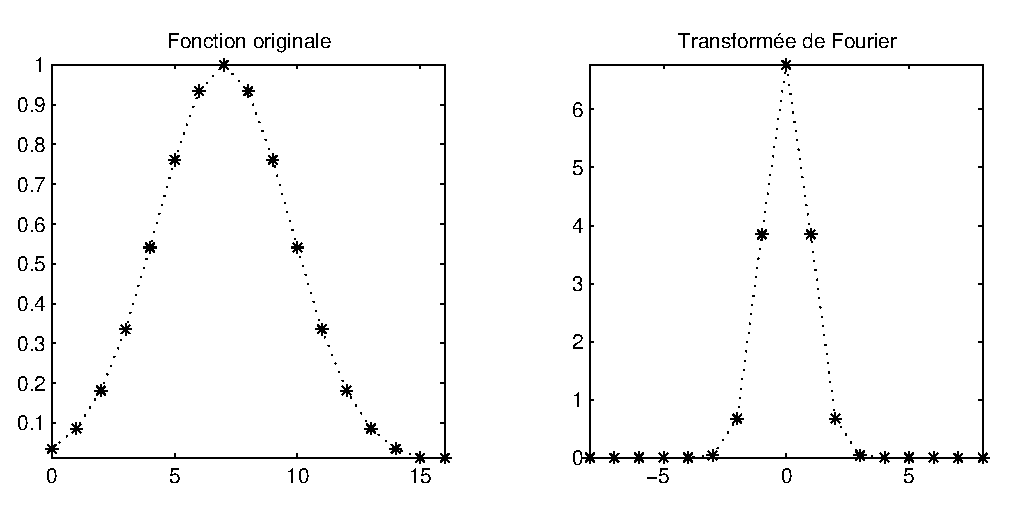
\includegraphics[scale = 0.7]{images/decomposition-fourier.eps}
    \end{center}
    \caption{Example of Fourier transform}
\label{fig-decomposition-fourier}
\end{figure}


\begin{rem}
The morphisms $ c $ and $\Ff $ are of course linear, so they are morphisms of vector spaces from $\CC[G]$ into $\CC[\wh{G}]$. They are in fact \textit{isomorphisms} of vector spaces, and to demonstrate this we will use the following Fourier inversion formula.
\end{rem}


\begin{prop}[Inversion formula]
\label{prop-decomposition-serie-fourier}
\index{Fourier!series} \index{Inversion!formula} For $ f \in \CC[G]$, we have the inversion formula
\begin{equation}
\label{eq-decomposition-serie-fourier-grpe-abelien}
f = \sum_{\chi \in \wh{G}}{c_f(\chi) \chi} = \frac{1}{|G|} \sum_{\chi \in \wh{G}}{\wh{f}(\chi) \chi^{-1}}.
\end{equation}

\end{prop}
\begin{proof}
The equation \eqref{eq-decomposition-serie-fourier-grpe-abelien} results immediately from the fact that $\wh{G}$ is an orthonormal basis of $\CC[G]$, by decomposing $f$ in this based.
\end{proof}


\begin{prop}[Fourier isomorphism]
$ c $ and $\Ff $ are isomorphisms of vector spaces from $\CC[G]$ into $\CC[\wh{G}]$.
\end{prop}
\begin{proof}
Let us show that $ c $ is injective. If $ c_f = 0 $, then the inversion formula \eqref{eq-decomposition-serie-fourier-grpe-abelien} shows that $ f = 0 $. As $G$ and $\wh{G}$ have the same cardinal (proposition \ref{cor-order-dual-equal-order-group}) the spaces $\CC[G]$ and $\CC[\wh{G}]$ have the same dimension $|G| = |\wh{G}|$. We therefore conclude that $ c $ is indeed an isomorphism. The reasoning is the same for $\Ff $.
\end{proof}


\begin{rem}
In reality, $\Ff $ is more than an isomorphism of vector spaces, since it also preserves a very particular algebra structure, the one defined by the convolution product. All this is the subject of Paragraph~\ref{sect2-convolution-transforme-fourier}.
\end{rem}
For now, let's continue to state the formulas that we get by using the decomposition in the base of characters.

\begin{prop}[Plancherel formula]
\label{prop-formula-floorel}
\index{Plancherel's formula} For $ (f, \, g) \in \CC[G]^2 $ we have the following formulas:
\begin{align}
\label{eq-formula-floorel-grpe-abelien-1}
\sum_{s \in G}{f (s) \ol{g (s)}} & = |G|\sum_{\chi \in \wh{G}}{c_{f}(\chi) \ol{c_{g}(\chi)}} \\
\label{eq-formula-floorel-grpe-abelien-2}
& = \frac{1}{|G|} \sum_{\chi \in \wh{G}}{\wh{f}(\chi) \ol{\wh{g}(\chi)}}.
\end{align}

\end{prop}
\begin{proof}
By decomposing $f$ and $g$ in the form $f(s) = \sum_{\chi \in \wh{G}}{c_{f}(\chi) \chi(s)}$ as well as $g(s) = \sum_{\chi \in \wh{G}}{c_{g}(\chi) \chi(s)}$, he comes
\begin{equation*}
\sum_{s \in G}{f (s) \ol{g (s)}} = |G|\dotp{f}{g} = |G|\sum_{(\chi_1, \, \chi_2) \in \wh{G}^2}{c_{f}(\chi_1) \ol{c_{g}(\chi_2)} \dotp{\chi_1}{\chi_2}}.
\end{equation*}
Hence the equation \eqref{eq-formula-floorel-grpe-abelien-1} using the orthogonality relations between characters. We prove in the same way the equation \eqref{eq-formula-floorel-grpe-abelien-2}.
\end{proof}


\begin{rem}{(\upshape \textbf{Link with theory $\mbold{L^2}$}).}
This formula is in every way similar to the formula that we obtain for the Fourier transform of two functions of $L^2(\RR)$. It translates the conservation of the scalar product (up to a constant) by the Fourier transform, since we can rewrite it in the form:
\begin{equation*}
\forall (f, \, g) \in \CC[G]^2, \quad \dotp{f}{g} = \frac{1}{|G|} \dotp{\wh{f}}{\wh{g}},
\end{equation*}
the second scalar product being of course that of $\CC[\wh{G}]$. This will be explained in detail in Section~\ref{sect1-link-trans-fourier-R}, where we discuss the link between the Fourier transform on the vectors of $\CC^N $ (called \textit{transform discrete}) and the Fourier transform \textit{continue}.
\end{rem}

% ------------------------------------------------- -----
% ------------------------------------------------- -----
% sub-section - Algebra of an abelian group
% ------------------------------------------------- -----
% ------------------------------------------------- -----
\subsection{Algebra of an abelian group}
\label{sect2-algebre-grpe-abelien}


\index{Product!term to term} \index{Convolution product} $G$ always designates a finite abelian group. Since the beginning of this talk, we have denoted $\CC[G]$ the (vector) space of functions from $G$ in $\CC$. We can give it an algebra structure thanks to the product of functions defined as follows:
\begin{equation}
\label{eq-defn-prod-term-term-functions}
\forall (f_1, \, f_2) \in \CC[G]^2, \; \forall g \in G, \quad (f_1 \cdot f_2)(g) \eqdef f_1(g) f_2(g).
\end{equation}
However, it is not this structure that will be useful for the following, but rather the one defined by the convolution product. Indeed, as we will see, the convolution product closely depends on the structure of the group $G$ considered, unlike the term-to-term product defined by the equation \eqref{sect2-convolution-transforme-fourier}. We will thus see in Paragraph~\ref{sect2-convolution-transforme-fourier} that the Fourier transform behaves in a very pleasant way for the convolution product.


\index{Algebra!of a group} We have already seen (to the proposition \ref{prop-base-c-g}) that a basis of the vector space $\CC[G]$ is given by the functions $\{\delta_g\}_{g \in G}$, where the function $\delta_G$, for $g \in G$, checks $\delta_g(g) = 1$ and $\delta_g(h) = 0 $ for $ h \in G$ such that $g \neq h$. Similarly, we have seen that a function $ f \in \CC[G]$ decomposes in the base $\{\delta_g\}_{g \in G}$ in
\begin{equation*}
f = \sum_{g \in G}{f(g) \delta_g}.
\end{equation*}
We then inject the group $G$ into the vector space $\CC[G]$ via the application
\begin{equation*}
j: g \in G \mapsto \delta_g \in \CC[G].
\end{equation*}
This allows to define (by structure transport) a multiplication noted $ *$ between the elements $\{\delta_g\}_{g \in G}$:
\begin{equation*}
\forall (g, \, h) \in G^2, \quad \delta_g * \delta_h \eqdef \delta_{g h}.
\end{equation*}
All that remains is to extend this multiplication to $\CC[G]$ by bilinearity in order to provide $\CC[G]$ with an algebra structure. This product is called the convolution product, and we can easily calculate the formula giving the expression of a product of two functions.

\begin{defn}[Convolution product]
\index{Convolution product} \label{notation-23} For $ f_1$ and $ f_2 $ two functions of $\CC[G]$, the convolution product $ f_1 * f_2 $ is given by
\begin{equation}
\label{eq-formula-prod-convol-grpe-abelien}
\forall g \in G, \quad (f_1 * f_2)(g) \eqdef \sum_{\scriptsize \begin{array}{c} (h, \, k) \in G^2 \\hk = g \end{array}}{f_1(h) f_2 (k)} = \sum_{h \in G}{f_1(h) f_2 (h^{-1} g)}.
\end{equation}

\end{defn}


\begin{rem}
For $ f \in \CC[G]$ we have
\begin{equation*}
\forall (g, \, h) \in G^2, \quad (f * \delta_g)(h) = f (h g^{-1}).
\end{equation*}
Thus the convolution by an element of $G$ (that is to say the convolution by a function $\delta_g$, using the identification) corresponds to a translation of the function. These properties will be explained again in the simple framework of $ G = \ZZ/n\ZZ$ in Section~\ref{sect1-tfd-prod-convol}. Let us content ourselves with stating the first properties of the convolution product.
\end{rem}


\begin{prop}
The convolution product is commutative, associative, and the map $ (f_1, \, f_2) \mapsto f_1 * f_2 $ is bilinear. We thus endow the vector space $\CC[G]$ with an algebra structure.
\end{prop}
\begin{proof}
The commutativity is easily verified by making the change of variable $ h'= h^{-1} g$ in the sum of the equation \eqref{eq-formula-prod-convol-grpe-abelien}. Associativity can be demonstrated by hand, or by using the \ref{thm-convolution-trans-fourier-grpe-abelien} theorem. The rest is easy.
\end{proof}
Before continuing, let's see \guill{graphically} what a convolution product looks like. Figure \figref{fig-convolution-intro} shows the convolution product with itself of a \guill{gate} function, on $\ZZ/16 \ZZ$. On the x-axis, we noted $\{0, \ldots, \, 15\}$ of the representatives of $\ZZ/16 \ZZ$. \begin{figure}[ht]
    \begin{center}
    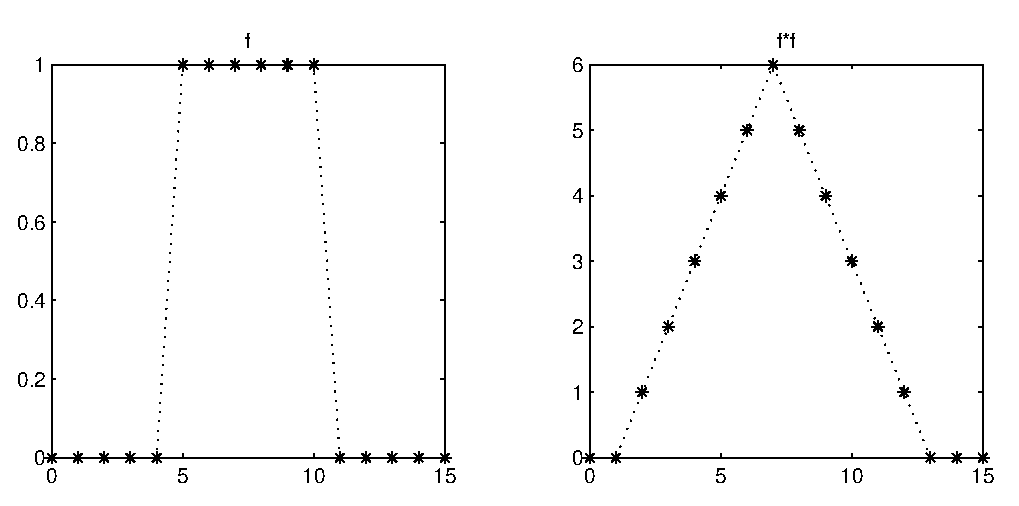
\includegraphics[scale = 0.7]{images/convolution-intro.eps}
    \end{center}
    \caption{Example of convolution calculation}
\label{fig-convolution-intro}
\end{figure}
This is the first time that we approach this kind of figures. These can be a bit confusing and the results aren't necessarily obvious. There are several possibilities. \begin{rs}
\item We can do the calculation by hand, and check that we get a \guill{triangle} function.
\item \index{Convolution!circular} We can expect the Section~\ref{sect1-tfd-prod-convol}, which studies in detail the discrete cyclic convolution. We will then be able to do the calculations with \Matlab{}, using the FFT algorithm.
\item We can read the Section~\ref{sect1-calculations-products}, which explains the link between the convolutional calculation and the multiplication of polynomials modulo $ X^n-1$.
\end{rs}


The fact that the convolution product is defined by extension of the product of the elements of $G$ allows us to state the following proposition.

\begin{prop}[Algebra morphism]
\label{prop-extension-morphism-grpe-algebra}
Let $\rho: G \rightarrow \CC^*$ be a group morphism. There is a unique way to extend it to an algebra morphism $\wt{\rho}: \CC[G] \rightarrow \CC$.
\end{prop}
\begin{proof}
Indeed, the construction of $\CC[G]$ tells us that $\wt{\rho}$ is only determined by the data of the values of $\wt{\rho}(\delta_g)$, for $ g \in G$. Now in the identification of $G$ as the canonical basis of $\CC[G]$, we have $\wt{\rho}(\delta_g) = \rho(g)$, which shows the uniqueness of the construction. It suffices then to show that the constructed morphism is indeed an algebra morphism. By definition of the convolution product, we can be satisfied with showing the conservation of the product over the elements $\{\delta_g\}_{g \in G}$, which is equivalent to the fact that $\rho$ is a morphism of group.
\end{proof}
This proposition tells us that there is a perfect correspondence between morphisms of groups of $G$ in $\CC^*$ and morphisms of algebras of $\CC[G]$ in $\CC$.

\begin{rem}{(\upshape \textbf{Probabilistic interpretation}).}
\label{rmk-interpretation-proba}
\index{Probability} The convolution product, which was introduced as the linear extension of a group operation, has a very important probabilistic interpretation. Let $ X $ and $ Y $ be two \textit{independent} random variables with values in a commutative finite group $G$. We denote by $ P_X $ and $ P_Y $ the corresponding probability distributions, that is to say $\forall g \in G, \; P_X(g) = \PP(\{X = g\})$. The fundamental result is that the probability distribution of the random variable $ X + Y $ is the convolution product of the distributions of $ X $ and $ Y $. This is therefore written $ P_{X + Y} = P_X * P_Y $. This theorem extends to continuous (with values in $\RR $) and discrete (with values in $\ZZ$) variables, provided that the appropriate convolution product is used. This result is very easy to show (the reader can verify it immediately), and we can consult \cite{ouvrard-2} on the applications of the convolution product in probability (in the continuous and discrete framework). The exercises \oldref{exo-repartition-proba} and \oldref{exo-marche-aleatoire} study the use of the Fourier transform on a finite group to solve probability problems.
\end{rem}

% ------------------------------------------------- -----
% ------------------------------------------------- -----
% sub-section - Convolution and Fourier transform
% ------------------------------------------------- -----
% ------------------------------------------------- -----
\subsection{Convolution and Fourier transform}
\label{sect2-convolution-transforme-fourier}


Let $G$ be a commutative finite group of order $n$. The following proposition shows that the definition of the Fourier transform is in fact very natural.

\begin{prop}[Algebra morphism]
\label{prop-thm-convol-fourier-grpe-finite}
Let $\chi \in \wh{G}$. The application
\begin{equation*}
\Ff_ \chi: \func{\CC[G]}{\CC}{f}{\wh{f}(\chi)}
\end{equation*}
corresponds to the unique way to extend the group morphism $\chi$ into an algebra morphism.
\end{prop}

\begin{proofnoqed}
The uniqueness results directly from the proposition \ref{prop-extension-morphism-grpe-algebra}. It only remains to show on the elements $\delta_G$ that $\Ff_ \chi$ corresponds to $\chi$, which is trivial:
\begin{equation*}
\forall g \in G, \quad \Ff_ \chi(\delta_g) = \sum_{x \in G}{\delta_g (x) \chi(x)} = \chi(g). \tag*{\qed}
\end{equation*}
\end{proofnoqed}

This property, which a posteriori justifies the introduction of the Fourier transform, is of capital importance, and we can summarize it in the form of the following convolution theorem.

\begin{thm}[Convolution and Fourier transform]
\label{thm-convolution-trans-fourier-grpe-abelien}
For $f$ and $g$ two functions of $\CC[G]$ we have
\begin{equation}
\label{eq-formula-convolution-functions-abelien-grpe}
\wh{f * g} = \wh{f} \cdot \wh{g} \quad \text{and} \quad c_{f * g} = |G| c_f \cdot c_g,
\end{equation}
where we denote by $\cdot $ the term-to-term product of two functions. The Fourier transform $\Ff $ is therefore an algebra isomorphism from $(\CC[G], \, *)$ to $(\CC[\wh{G}], \, \cdot)$.
\end{thm}



\index{Determinant!circulating} This convolution property is undoubtedly the
most used property of the Fourier transform, since it allows to change a rather
complex problem (the computation of a convolution of two functions) into a more
simple one (the calculation of the product term by term). The occurrences of this principle of simplification will be numerous throughout the book, whether they are theoretical studies (calculation of circulating determinant, Poisson's formula, etc.) or much more applied (filtering, product of large integers, decoding corrective codes, etc.).
% ------------------------------------------------- -----
% ------------------------------------------------- -----
% ------------------------------------------------- -----
% section - Exercises
% ------------------------------------------------- -----
% ------------------------------------------------- -----
% ------------------------------------------------- -----
\section{Exercises}
% \addcontentsline{toc}{section}{Exercises}
\label{sect1-chap1-exercises}

\begin{exo}[Circulating determinant]
\label{exo-determinant-circulating}

\index{Determinant!circulating} Let $G$ be a cyclic group. We fix $f \in \CC[G]$. We want to calculate the determinant of endomorphism
\begin{equation*}
\Phi^f \func{\CC[G]}{\CC[G]}{u}{f * u}.
\end{equation*}
We will often meet this type of application, in particular in Paragraph~\ref{sec2-linear-filters}, where it will be question of filtering. \begin{enumerate}
\item Explain why the elements $\chi \in \wh{G}$ are eigenvectors of $\Phi^f $. What are the associated eigenvalues?
\item What is the matrix $A$ of the endomorphism $\Phi^f $ in the base $\{\delta_g\}_{g \in G}$ of $\CC[G]$? Deduce from the previous question an expression of $\det (A)$.
\item By judiciously choosing the group $G$ and the application $f$, show that we have
\begin{equation*}
\det \begin{pmatrix} a_0 & a_1 & a_2 & \ldots & a_{n-1} \\a_{n-1} & a_0 & a_1 & \ldots & a_{n-2} \\vdots & \vdots & \vdots & & \vdots \\a_1 & a_2 & a_3 & \ldots & a_{0} \end{pmatrix} = \prod_{i = 0}^{n-1} \left(\sum_{j = 0}^{n-1}{a_j} \omega^{ij} \right),
\end{equation*}
where $ (a_0, \ldots, \, a_{n-1}) \in \CC^n $, and $\omega \eqdef e^{\frac{2 \imath \pi}{n}}$ (A such determinant is called \textit{circulating determinant}).
\item After having read the chapter \oldref{chap-tfd} devoted to the discrete Fourier transform and the FFT algorithm, propose a fast implementation of the circulating determinant calculus.
\end{enumerate}
\end{exo}


\begin{exo}[Dual of $\mbold{SO(3)}$]
\label{exo-dual-so3}

\index{Rotation} We denote by $SO(3)$ the group of real, orthogonal $ 3 \times 3 $ matrices with determinant 1. It corresponds to the rotations of $\RR^3 $. We want to show that $SO(3)$ has no non-trivial character. \begin{enumerate}
\item Show that two rotations of the same angle are conjugate.
\item Let $\chi$ be an element of the dual of $ SO(3)$. For $g \in SO(3)$, show that $\chi(g)$ depends only on the angle of $g$.
\item We denote by $r_{\alpha}$ the angle rotation $\alpha$ around $ (1, \, 0, \, 0)$, and $ s_{\alpha}$ the angle rotation $\alpha$ around $ (0, \, 1, \, 0)$. We consider $t_{\beta} \eqdef r_{\alpha} s_{\alpha}^{-1}$. Show that $t_{\beta}$ is a rotation of some angle $\beta $, and that when $\alpha$ traverses $[0, \, \pi]$, then $\beta $ does the same.
\item Deduce that $\chi = $ 1.
\end{enumerate}
\end{exo}


\begin{exo}[Enumeration of solutions]
\label{exo-enombrement-solutions}

\index{Enumeration} Let G be a finite abelian group, and a function $\varphi: G^n \rightarrow G$. For $ h \in G$, we denote by $ N(h)$ the number of $n$ -uples $ (g_1, \ldots, \, g_n)$ such that $\varphi (g_1, \ldots, \, g_n ) = h $. Show that we have
\begin{equation*}
N(h) = \frac{1}{|G|} \sum_{g_1 \in G}{\cdots \sum_{g_n \in G}{\sum_{\chi \in \wh{G}}{\chi \left(\varphi (g_1, \ldots, \, g_n) \right) \ol{\chi}(h)}}}.
\end{equation*}

\end{exo}


\begin{exo}[Indicator functions]
\label{exo-indicator-functions}

\index{Function!indicator} Let $G$ be a finite abelian group and $ A \subset G$. We denote by $ f_A $ the indicator function of $A$. \begin{enumerate}
\item Show that
\begin{equation*}
\norm{f_A}_2 = \sqrt{\frac{|A|}{|G|}} \quad \quad \text{et} \quad \quad \wh{f_A}(\chi_0) = |A|,
\end{equation*}
where we noted $\chi_0 $ the trivial character.
\item We assume that $|A|\leq \frac{1}{2}|G|$. We define
\begin{equation}
\label{eq-defn-phi-ensemble}
\Phi(A) \eqdef \max \enscond{|\wh{f_A}(\chi)|}{\chi \in \wh{G}, \; \chi \neq \chi_0}.
\end{equation}
Show that we have
\begin{equation}
\label{eq-ineq-regularity-function-indic}
\sqrt{\frac{|A|}{2}} \leq \Phi(A) \leq |A|.
\end{equation}

\item We take the case where $|A| > \frac{1}{2}|G|$. Show that we have $\Phi(A) = \Phi(G \backslash A)$, where we have denoted $ G \backslash A $ the complement of $A$ in $G$. Deduce a lowering of $\Phi(A)$ similar to \eqref{eq-ineq-regularity-function-indic}.
\item Show that if $\alpha$ is an automorphism of $G$, then $\Phi(\alpha (A)) = \Phi(A)$.
\end{enumerate} Intuitively, the closer $\Phi(A)$ is to the lower bound, the more the elements of $A$ are evenly distributed in $G$. The exercise \oldref{exo-repartition-proba} studies and quantifies this phenomenon. We can see an analogy with the study of the Fourier transform of a continuous function: the lower the high frequency Fourier coefficients, the more \guill{smooth} the function. These indicator functions will be used in Section~\ref{sect1-applications-correctors-codes} in the context where $A$ is used as corrective code. Once again, it is the spectral properties of $ f_A $ that will be used to study the \guill{geometry} of the set $A$.
\end{exo}


\begin{exo}[Equations on a finite abelian group]
\label{exo-eqn-grpe-abelien-finite}

\index{Equation!on an abelian group} This exercise uses the notations and results of exercise \oldref{exo-indicator-functions}. It is taken from the review article by Babai{\upshape \cite{babai-fourier-equations}}. \begin{enumerate}
\item We consider $ A_1, \ldots, \, A_k \subset G$, and we study the equation
\begin{equation}
\label{eq-exo-nbr-solution-eqn-grpe-finite}
x_1 + \cdots + x_k = a \quad \quad \text{with} \quad x_i \in A_i, \quad i = 1, \ldots, \, k.
\end{equation}
Explain how we can be reduced to the case $ a = 0 $. We denote by $n$ the number of solutions of \eqref{eq-exo-nbr-solution-eqn-grpe-finite}, in the case $ a = 0 $. Using the result of the exercise \oldref{exo-enombrement-solutions}, show that
\begin{equation*}
N = \frac{1}{|G|} \sum_{\chi \in \wh{G}}{\sum_{x_i \in A_i}{\chi(x_1 + \cdots + x_k)}} = \frac{| A_1 |\cdots | A_k |}{|G|} + R,
\end{equation*}
with
\begin{equation*}
R \eqdef \frac{1}{|G|} \sum_{\chi \neq \chi_0}{\prod_{i = 1}^k{\wh{f_{A_i}}(\chi)}}.
\end{equation*}

\item \index{Cauchy-Schwartz inequality} We assume that $ k = 3 $. To show that
\begin{equation*}
| R |\leq \frac{\Phi(A_3)}{|G|} \sum_{\chi \in \wh{G}}{|\wh{f_{A_1}}(\chi) | |\wh{f_{A_2}}(\chi) |} \leq \Phi(A_3) \sqrt{| A_1 | | A_2 |},
\end{equation*}
where $\Phi $ is defined by the equation \eqref{eq-defn-phi-ensemble} (we can use the Cauchy-Schwartz inequality). Show, using the result of the exercise \oldref{exo-indicator-functions}, question 4., that this is still valid when $ a \neq 0 $.
\item Deduce that if
\begin{equation*}
\frac{\Phi(A_3)}{| A_3 |} <\frac{\sqrt{| A_1 | | A_2 |}}{|G|},
\end{equation*}
then the equation $ x_1 + x_2 + x_3 = a $, with $ x_i \in A_i $, $ i = 1, \, 2, \, 3 $, has at least one solution.
\end{enumerate} This surprising result therefore tells us that if at least one of the three sets $ A_i $ is well distributed, and if the three sets are sufficiently large, then the considered equation has at least one solution. The exercise \oldref{exo-thm-fermat-finite-body} applies this result to $ G = \FF_q $ to study Fermat's theorem on finite fields.
\end{exo}


\begin{exo}[Heisenberg group]
\label{exo-groupe-heisenberg}

\index{Heisenberg's!group} Let $G$ be a finite abelian group. We denote by $\Uu $ the group of complex numbers of modulus $ 1$. We denote by $\Hh(g) \eqdef \Uu \times G \times \wh{G}$ provided with the operation
\begin{equation*}
(\lambda, \, x, \, \chi) \cdot(\mu, \, y, \, \tau) =(\lambda \mu \tau (x), \, xy, \, \chi \tau )
\end{equation*}
the Heisenberg group associated with $G$. \begin{enumerate}
\item Show that we define a group structure in this way. In particular, what is the neutral element and what is the inverse of a generic element $(\lambda, \, x, \, \chi) \in \Hh(g)$?
\item Show that we can define an action of $\Hh(g)$ on $\CC[G]$ by setting
\begin{equation*}
\forall f \in \CC[G], \; \forall(\lambda, \, x, \, \chi) \in \Hh(g), \quad(\lambda, \, x, \, \chi) \cdot f: z \mapsto \lambda \chi( z) f (xz).
\end{equation*}

\item \index{Translation} For $(\lambda, \, x, \, \chi) \in \Hh(g)$ and $ f \in \CC[G]$, we define respectively the expansion operators, translation, and modulation by
\begin{equation*}
D_ \lambda (f) (z) = \lambda f (z), \quad \quad T_x (f) (z) = f (xz), \quad \quad M_ \chi(f) (z) = \chi(z) f (z).
\end{equation*}
Express the action of $\Hh(g)$ on $\CC[G]$ in terms of these three operators. How do these three operators behave with respect to the Fourier transform defined in the equation \eqref{eq-transf-fourier-grpe-abelien}? What is the link with the continuous Fourier transform on $\RR $?
\item \index{Bidual} By canonically identifying $G$ to $\whwh{G}$ as described in Paragraph~\ref{sect2-bidual}, how the product on $\Hh(\wh{G}) = \Uu \times \wh{G} \times G$ defined? How to define an action of $\Hh(\wh{G})$ on $\CC[\wh{G}]$?
\item We define the function
\begin{equation*}
\alpha: \func{\Hh(g)}{\Hh(\wh{G})}{(\lambda, \, x, \, \chi)}{(\lambda \chi^{-1} ( x), \, \chi, \, x^{-1})}.
\end{equation*}
Show that $\alpha$ is an isomorphism of groups, and that we have
\begin{equation*}
\forall f \in \CC[G], \; \forall(\lambda, \, x, \, \chi) \in \Hh(g), \quad \Ff \left((\lambda, \, x, \, \chi) \cdot f \right) = \alpha(\lambda, \, x, \, \chi) \cdot \Ff (f),
\end{equation*}
where $\Ff $ denotes the Fourier transform defined in the equation \eqref{eq-transf-fourier-grpe-abelien}.
\item \index{Lemma!of Schur} We suppose that $\Phi: \CC[G] \rightarrow \CC[G]$ commutes with the action of $\Hh(g)$, that is say that
\begin{equation*}
\forall f \in \CC[G], \; \forall(\lambda, \, x, \, \chi) \in \Hh(g), \quad \Phi((\lambda, \, x, \, \chi) \cdot f) =(\lambda, \, x, \, \chi) \cdot \Phi(f).
\end{equation*}
Show that there exists $ r \in \CC^*$ such that $\forall f \in \CC[G], \; \Phi(f) = r f $. We can reason on the matrix of $\Phi $ expressed in the base $\{\delta_g\}_{g \in G}$ of $\CC[G]$, or then use Schur's lemma \ref{lemma-schur}. What happens if $\Phi: \CC[G] \rightarrow \CC[\wh{G}]$ switches the actions of $\Hh(g)$ and $\Hh(\wh{G})$?
\end{enumerate}
\end{exo}


\begin{exo}[Fourier transform and orthogonalization]
\label{exo-series-fourier-orthogonalisation}

\index{Orthogonalization} \index{Translation} We consider a function $ f \in L^2(\RR)$. We denote by $\tau_r $ the translation of $ r $ on $L^2(\RR)$, i.e. $\tau_r (f) = f(\cdot-r)$. \begin{enumerate}
\item Show that the family $\{\tau_n (f)\}_{n \in\ZZ}$ is orthonormal if and only if
\begin{equation*}
\text{for a.e. } \omega \in \RR, \quad \sum_{k \in\ZZ}{|\wh{f}(\omega + 2k \pi) |^2} = 1,
\end{equation*}
where we have denoted $\wh{f} \in L^2(\RR)$ the Fourier transform of $f$, defined, for the functions $ f \in L^1(\RR)$ by
\begin{equation*}
\text{for a.e. } \omega \in \RR, \quad \wh{f}(\omega) \eqdef \int_{\RR}{f (x) e^{- \imath \omega x} \d x},
\end{equation*}
and extended by density to $L^2(\RR)$ whole.
\item \label{notation-24} We assume that there exists $ A> 0 $ such that
\begin{equation*}
\text{for a.e. } \omega \in \RR, \quad A \leq \sum_{k \in\ZZ}{|\wh{f}(\omega + 2k \pi) |^2}.
\end{equation*}
Show that if we denote by $\varphi $ the function of $L^2(\RR)$ such that
\begin{equation*}
\text{for a.e. } \omega \in \RR, \quad \wh{\varphi}(\omega) \eqdef \frac{\wh{f}(\omega)}{\left(\sum_{k \in\ZZ}{|\wh{f}(\omega + 2k \pi) |^2} \right)^{1/2}},
\end{equation*}
then the family $\{\tau_n(\varphi)\}_{n \in\ZZ}$ is orthonormal (equalities are to be considered for almost all $\omega $).
\end{enumerate} The following exercise \oldref{exo-orthogonalization-abelian-group} proposes to study the same orthogonalization problem, but within the framework of a finite abelian group.
\end{exo}

\begin{exo}[Orthogonalization on an abelian group]
\label{exo-orthogonalization-abelian-group}

\index{Orthogonalisation} \index{Transformation!group} \index{Unitary!endomorphism} This exercise is inspired by the article by \nompropre{Bernardini} and \nompropre{Kovacevic}{\upshape \cite{bernardini-orthogonalisation-1}}. Let $ V $ be a $\CC$ -vector space of dimension $n$, endowed with a Hermitian product $\dotp{\cdot}{\cdot}$. Let $G$ be a finite abelian group of unit transformations of $ V $, and let $ b \in V $. We say that $ b $ is orthonormal for the action of $G$ on $ V $ if the set $ G_b \eqdef \enscond{A b}{A \in G}$ is orthonormal. This means that
\begin{equation*}
\forall (x, \, y) \in G_b^2, \quad \dotp{x}{y} = \delta_x^y.
\end{equation*}
\begin{enumerate}
\item We note
\begin{equation*}
\psi_b: \func{G}{\CC}{A}{\dotp{A b}{b}}.
\end{equation*}
Show that $ b $ is orthonormal for the action of $G$ if and only if $\wh{\psi_b} \equiv 1$, i.e. if and only if $\forall \chi \in \wh{G}$, $|G|\dotp{\Uu_ \chi b}{b} = $ 1, where we noted
\begin{equation*}
\forall \chi \in \wh{G}, \quad \Uu_ \chi \eqdef \frac{1}{|G|} \sum_{A \in G}{\chi(A) A} \quad \in \Ll (V, V).
\end{equation*}

\item Show that the operators $\Uu_ \chi$ are orthogonal projectors, and that they are two by two orthogonal, that is to say
\begin{equation*}
\forall(\chi_1, \, \chi_2) \in \wh{G}^2, \quad \Uu_{\chi_1} \Uu_{\chi_2} = \left\{\begin{array}{lll} 0 & \text{if} & \chi_1 \neq \chi_2 \\\Uu_{\chi_1} & \text{if} & \chi_1 = \chi_2 \end{array} \right.,
\end{equation*}
and $\Uu_ \chi^* = \Uu_ \chi$ ($ A^*$ denotes the assistant of $A$).
\item We assume that $\wh{\psi_b}$ does not vanish. We notice
\begin{equation*}
\wt{b} \eqdef \sum_{\chi \in \wh{G}}{\frac{1}{\sqrt{\wh{\psi_b}(\chi)}} \Uu_ \chi b},
\end{equation*}
where $\sqrt{\wh{\psi_b}(\chi)}$ denotes one of the two possible roots. Show that $\wt{b}$ is orthonormal for the action of $G$.
\item What connection can we make with the exercise \oldref{exo-series-fourier-orthogonalisation}?
\end{enumerate} For a more in-depth study of this method in the case of cyclic groups $\ZZ/n\ZZ$, we can look at the exercise \oldref{exo-series-fourier-orthogonalisation}.
\end{exo}


\begin{exo}[Distribution of probability]
\label{exo-repartition-proba}

\index{Probability} Let $G$ be a finite abelian group, and $ P: G \rightarrow \RR^+ $ the distribution function of a probability law on $G$, which means that $\sum_{g \in G}{P(g)} = $ 1. We denote by $ U $ the uniform distribution, that is to say $ U(g) = \frac{1}{|G|}$ for all $ g \in G$. We denote by $\chi_0 $ the trivial character of $G$. \begin{enumerate}
\item Calculate $\wh{P}(\chi_0)$ as well as $\wh{U}(\chi)$, for $\chi \in \wh{G}$. Deduce an expression of $\norm{P - U}_2^2 $.
\item Show that we have
\begin{equation*}
\forall g \in G, \quad \left| P(g) - \frac{1}{|G|} \right|^2 \leq \frac{1}{|G|} \sum_{\chi \neq \chi_0}{|\wh{P} ( \chi) |^2}.
\end{equation*}

\end{enumerate} In a way, the quantity $\norm{P - U}_2^2 $ measures the uniformity of the distribution $ P $, and as we have already seen for the characteristic functions (exercise \oldref{exo-indicator-functions}), this is characterized by the Fourier coefficients $\wh{P}(\chi)$, for $\chi \neq \chi_0 $.
\end{exo}


\begin{exo}[Random walk]
\label{exo-marche-aleatoire}

\index{Random walk} \index{Probability} \index{Markov chain} \index{Transition matrix} We consider a random walk on $\ZZ/n\ZZ$ cons \-trui \-te as follows. The random variable $ X_k \in\ZZ/n\ZZ$ designates a position on the circle $\ZZ/n\ZZ$ at the instant $ k \in \NN $. The displacement between the instant $ k $ and $ k + 1$ is given by a transition probability $ p_{i, j} \eqdef \PP (X_{k + 1} = j \, |\, X_k = i )$. \begin{enumerate}
\item We denote by $ p^{(k)}: G \rightarrow [0, \, 1]$ the probability distribution of $ X_k $, i.e. for $0 \leq i <n $, $ p^{(k)} (i) = \PP (X_k = i)$. We can also write $ p^{(k)}$ in the form of a vector of size $n$. Show that $ p^{(k + 1)} = P p^{(k)}$, where we have denoted $ P $ the transition matrix $\{p_{i, j}\}_{0 \leq i, j \leq n-1}$. Deduce that $ p^{(k)} = P^kp^{(0)}$, where $ p^{(0)} = \{1, \, 0, \ldots, \, 0\}$ is the initial distribution.
\item Let $0 <p <1$. We consider the simplest random walk, given by
\begin{equation*}
\left\{\begin{array}{l} p_{i, i-1} = p, \quad \quad p_{i, i + 1} = 1-p, \\p_{i, j} = 0 \quad \text{if} \quad i \notin \{i-1, \, i + 1\} \end{array} \right. .
\end{equation*}
Show that we then have $ P x = v * x $, where $ *$ denotes the product of convolution and $ v = \{0, \, p, \, 0, \ldots, \, 0, \, 1-p\}$. How can we find this result by considering sums of random variables, and by using the remark \ref{rmk-interpretation-proba}?
\item Express the Fourier transform $\wh{p^{(k)}}$ from $\wh{p^{(0)}}$. Deduce that if $n$ is odd, then
\begin{equation*}
p^{(k)} \tv{k \to \pinf} u \quad \quad \text{where} \quad \quad u \eqdef \{1/n, \ldots, \, 1/n\}.
\end{equation*}
What happens if $n$ is even?
\item \index{Translation} Generalize this result to a translation invariant random walk, that is to say such that
\begin{equation*}
p_{i, j} = v_{j-i} \quad \quad \text{with} \quad \quad v \in ([0, \, 1])^n.
\end{equation*}

\end{enumerate} The figure \figref{fig-marche-aleatoire} shows the progression of the probability distribution $ p^{(k)}$ in the case of two random walks. We see that the second step converges more quickly towards the uniform distribution (we can make the link with the size of the Fourier coefficients). \begin{figure}[ht]
    \begin{center}
    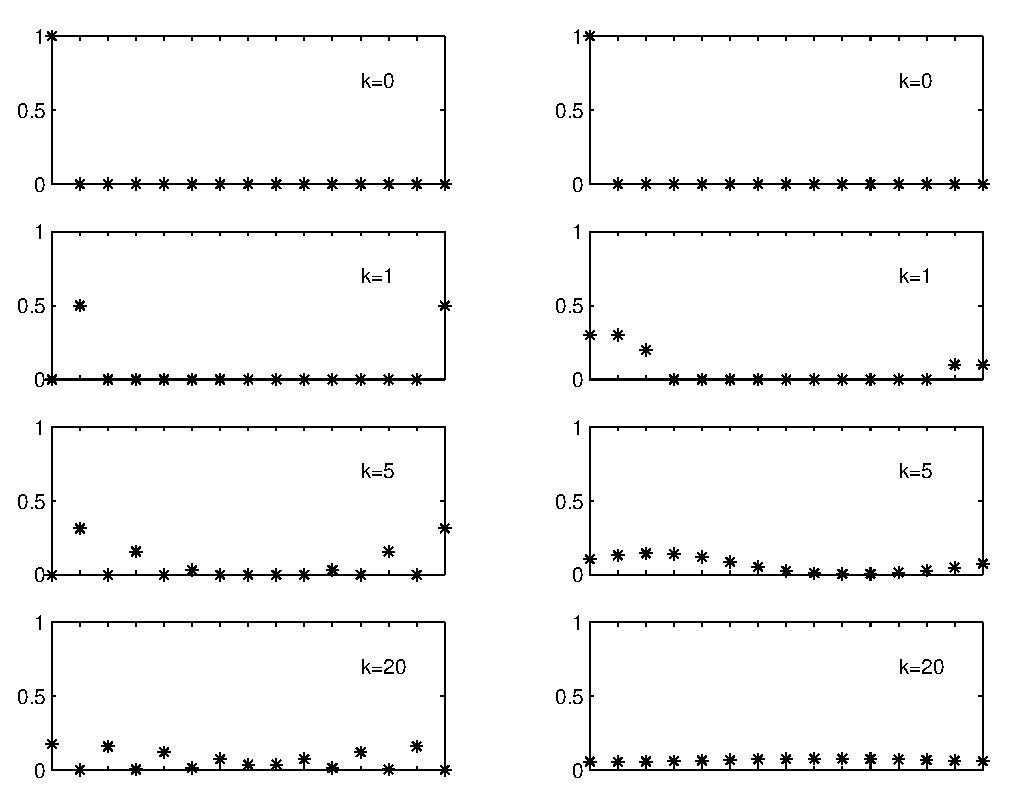
\includegraphics[scale = 0.6]{images/marche-aleatoire.eps}
    \end{center}
    \caption{Random walks for the transition probabilities $\{0, \, 1/2, \, 0, \ldots, \, 0, \, 1/2\}$ (left) and $\{0.3, \, 0.3, \, 0.2, \, 0, \ldots, \, 0, \, 0.1, \, 0.1\}$ (right)}
\label{fig-marche-aleatoire}
\end{figure}

\end{exo}


\begin{exo}[Discrete uncertainty principle]
\label{exo-principle-uncertainty-discrete}

\index{Uncertainty!principle} \index{Uncertainty} \index{Support} 
Let $G$ be a finite group, and $ f \in \CC[G]$ a non-zero function. We want to show that we have
\begin{equation}
	\label{eq-pcpe-uncertainty-discrete}
\big |\Supp (f) \big |\times \big |\Supp \big(\wh{f} \big) \big |\geq |G|,
\end{equation}
where $|\Supp (f) |$ denotes the size of the support of $f$. 
\begin{enumerate}
\item We consider, first of all, the group $ G = \ZZ/n\ZZ$. Show that if $f$ has $ p $ non-zero elements, then $\wh{f}$ cannot have $ p $ consecutive zeros. Deduce the equation \eqref{eq-pcpe-uncertainty-discrete}. This result was demonstrated first by \nompropre{Donoho} and \nompropre{Stark}{\upshape \cite{donoho-stark-uncertainty}}.
%%
\item \index{Cauchy-Schwartz inequality!} We return to the general case of a finite abelian group $G$. \\We denote by $ M \eqdef \sup \enscond{f (x)}{x \in G}$ and $\norm{f}_2^2 \eqdef \dotp{f}{f}$. To show that
\begin{equation*}
\norm{f}_2^2 \leq \frac{M^2}{|G|}|\Supp (f) |\quad \quad \text{et} \quad \quad M \leq \frac{1}{|G|} \sum_{\chi \in \wh{G}}{|\wh{f}(\chi) |}.
\end{equation*}
Using the Cauchy-Schwartz inequality, deduce that
\begin{equation*}
M^2 \leq \frac{|\Supp(\wh{f}) |}{|G|} \norm{\wh{f}}_ 2^2, \quad \quad \text{then,} \quad \quad M^2 \leq \norm{f}_2^2 |\Supp(\wh{f}) |.
\end{equation*}
To conclude that
\begin{equation*}
\norm{f}_2^2 \leq \frac{\norm{f}_2^2}{|G|}|\Supp (f) |\times |\Supp(\wh{f}) |.
\end{equation*}
%%%
\item \index{Subgroup} \index{Orthogonal!of a subgroup} Let $ H \subset G$, a subgroup and $ f_H \in \CC[G]$, its characteristic function. Show that we have
\begin{equation*}
\wh{f_H} = |H| f_{H^\sharp},
\end{equation*}
where we denote by $ H^\sharp \subset \wh{G}$ the orthogonal of $H$. Deduce that the function $f$ reaches the bound of the equation \eqref{eq-pcpe-uncertainty-discrete}. In fact, we can show that any function which reaches this bound is related to such a function $ f_H $ by a translation and a dilation. This is demonstrated in the article by \nompropre{Matusiak}{\upshape \cite{matusiak-donoho-stark}}.
\end{enumerate} 
This conclusion on the localization of temporal and frequency supports may seem negative at first glance: it prohibits us from constructing signals well localized both in time and in frequency. However, it can be used to advantage, for example to build efficient corrective codes, as the proposition \ref{prop-dist-minimal-code-bch} will show.
\end{exo}
